\documentclass{article}

\usepackage{graphicx}
\usepackage{tikz}
\usepackage{tikzsymbols}
\usetikzlibrary{calc,patterns,shapes.geometric}
\pagestyle{empty}
\usepackage[margin=0pt]{geometry}
\geometry{papersize={14in,12in}}

\def\centerarc[#1](#2)(#3:#4:#5){\draw[#1] ($(#2)+({#5*cos(#3)},{#5*sin(#3)})$) arc (#3:#4:#5);}

\begin{document}
	\begin{figure}
		\centering
		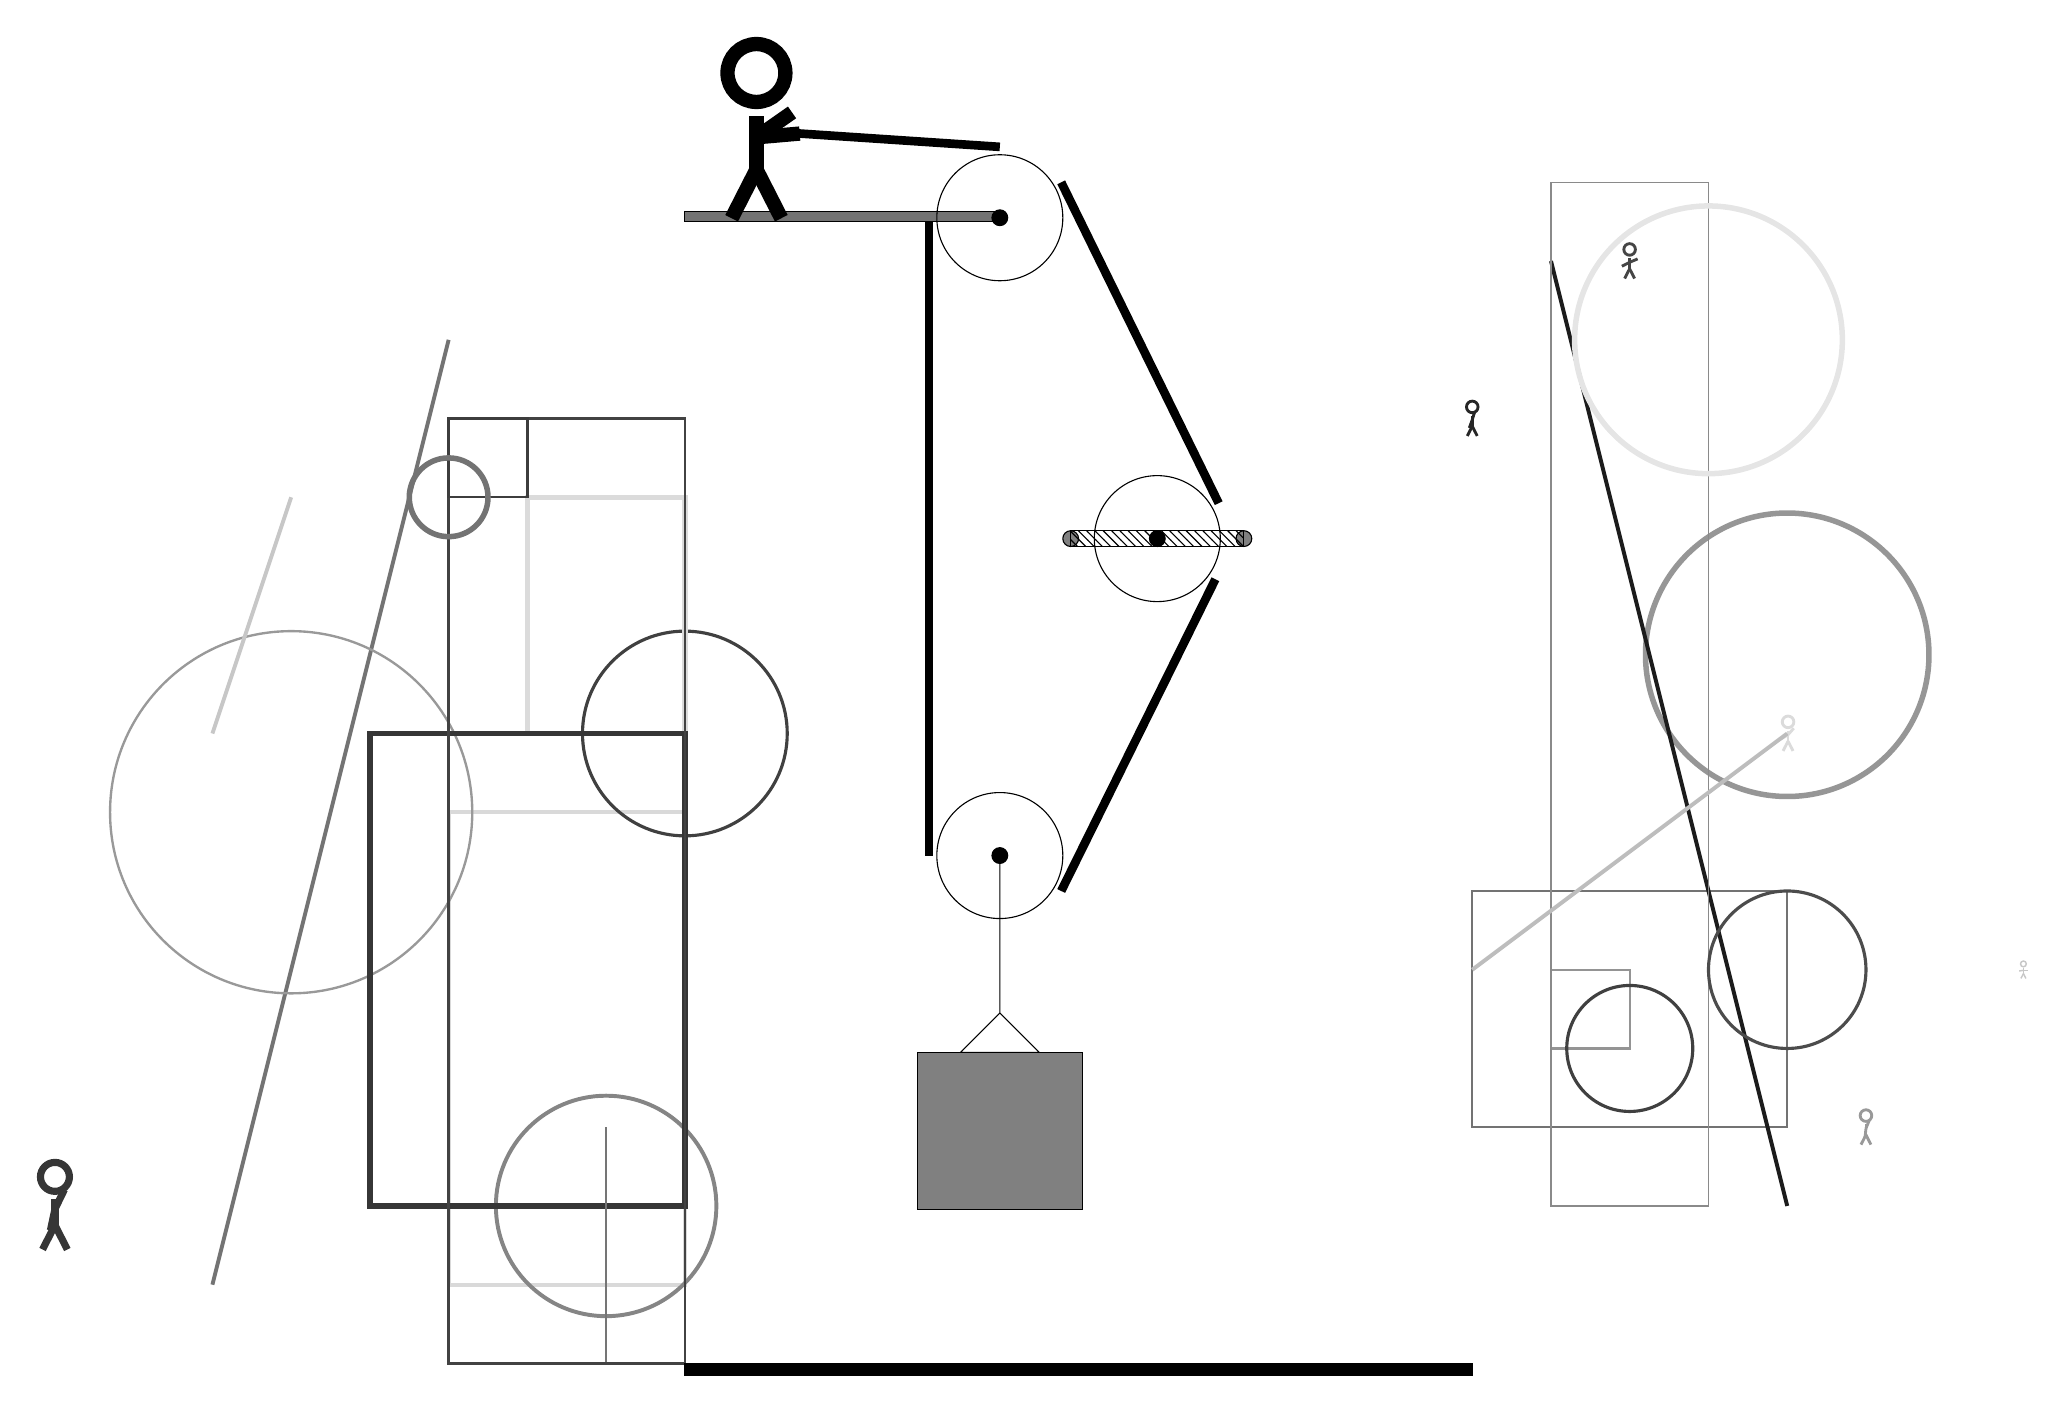
\begin{tikzpicture}
			%%%%% START %%%%%
			
			\draw[fill=black!55] (-2, 11.5) rectangle (2, 11.625);
			
			\draw (2, 3.45) circle (0.8);
			\draw[fill=black] (2, 3.45) circle (0.1);
			
			\draw (2, 11.55) circle (0.8);
			\draw[fill=black] (2, 11.55) circle (0.1);
			
			\draw [line width=0.7mm, color=black!41](12, 6) circle (1.8);
			
			\draw[line width=0.2mm, color=black!55] (8, 0) rectangle (12, 3);
			\draw[line width=0.5mm, color=black!55](-5, 10) -- (-8, -2);
			\node[line width=0.5mm, color=black!40] at (13, 0) {\Strichmaxerl[2][84][68]};
			\draw [line width=0.3mm, color=black!42](-6, 3) circle (0.0);
			\draw[line width=0.3mm, color=black!42] (10, 1) rectangle (9, 2);
			
			\draw [line width=0.4mm, color=black!75](10, 1) circle (0.8);
			\node[line width=0.6mm, color=black!85] at (8, 9) {\Strichmaxerl[2][70][73]};
			\draw[line width=0.5mm, color=black!15] (-2, -2) rectangle (-5, 4);
			\node[line width=0.6mm, color=black!22] at (15, 2) {\Strichmaxerl[1][9][0]};
			\draw [line width=0.5mm, color=black!48](-3, -1) circle (1.4);
			\draw[line width=0.5mm, color=black!89](12, -1) -- (9, 11);
			\draw [line width=0.4mm, color=black!75](-2, 5) circle (1.3);
			
			\draw [line width=0.3mm, color=black!40](-7, 4) circle (2.3);
			\draw[line width=0.2mm, color=black!46] (9, -1) rectangle (11, 12);
			\node[line width=0.7mm, color=black!79] at (-10, -1) {\Strichmaxerl[5][78][64]};
			
			\node[line width=0.6mm, color=black!73] at (10, 11) {\Strichmaxerl[2][27][23]};
			\node[line width=0.5mm, color=black!14] at (12, 5) {\Strichmaxerl[2][31][49]};
			\draw[line width=0.7mm, color=black!14] (-2, 8) rectangle (-4, 5);
			\draw[line width=0.7mm, color=black!79] (-2, -1) rectangle (-6, 5);
			\draw[line width=0.5mm, color=black!26](12, 5) -- (8, 2);
			
			\draw[line width=0.5mm, color=black!22](-7, 8) -- (-8, 5);
			\draw [line width=0.7mm, color=black!10](11, 10) circle (1.7);
			\draw[line width=0.3mm, color=black!54] (-3, -3) rectangle (-3, 0);
			\draw [line width=0.4mm, color=black!70](12, 2) circle (1.0);
			
			\draw[line width=0.3mm, color=black!74] (-2, 9) rectangle (-5, -3);
			
			\draw[line width=0.3mm, color=black!76] (-4, 8) rectangle (-5, 9);
			\draw [line width=0.7mm, color=black!55](-5, 8) circle (0.5);
			
			\draw[fill=white](4, 7.475) circle (0.8);
			\draw[fill=black] (4, 7.475) circle (0.1);
			\draw[fill=black!50] (2.9, 7.475) circle (0.1);
			\draw[fill=black!50] (5.1, 7.475) circle (0.1);
			\draw[pattern=north west lines, pattern color=black] (2.9, 7.575) rectangle (5.1, 7.375);
			
			\draw (2, 3.45) -- (2, 1.45) -- (1.5, 0.95) -- (2.5, 0.95) -- (2, 1.45);
			\draw[fill=black!50] (0.95, 0.95) rectangle (3.05, -1.05);
			
			\draw[line width=1.1mm] (1.1, 11.5) -- (1.1, 3.45);
			\centerarc[line width=1.1mm](2, 3.45)(180:330:0.9);
			\draw[line width=1.1mm](2.7794, 3.0) -- (4.7373, 6.9588);
			\centerarc[line width=1.1mm](4, 7.475)(390:325:0.9);
			\draw[line width=1.1mm](4.7794, 7.925) -- (2.7794, 12.0);
			\centerarc[line width=1.1mm](2, 11.55)(30:90:0.9);
			\draw[line width=1.1mm](2, 12.45) -- (-1, 12.65);
			
			\node at (-1, 12.65) {\Strichmaxerl[10][-175][35]};
			
			\draw[fill=black] (-2, -3) rectangle (8, -3.15);
			
			%%%%% END %%%%%
		\end{tikzpicture}
	\end{figure}	
\end{document}